\begin{figure}[htbp]
  \centering

  \begin{subfigure}[t]{0.48\textwidth}
    \vspace{0pt}
    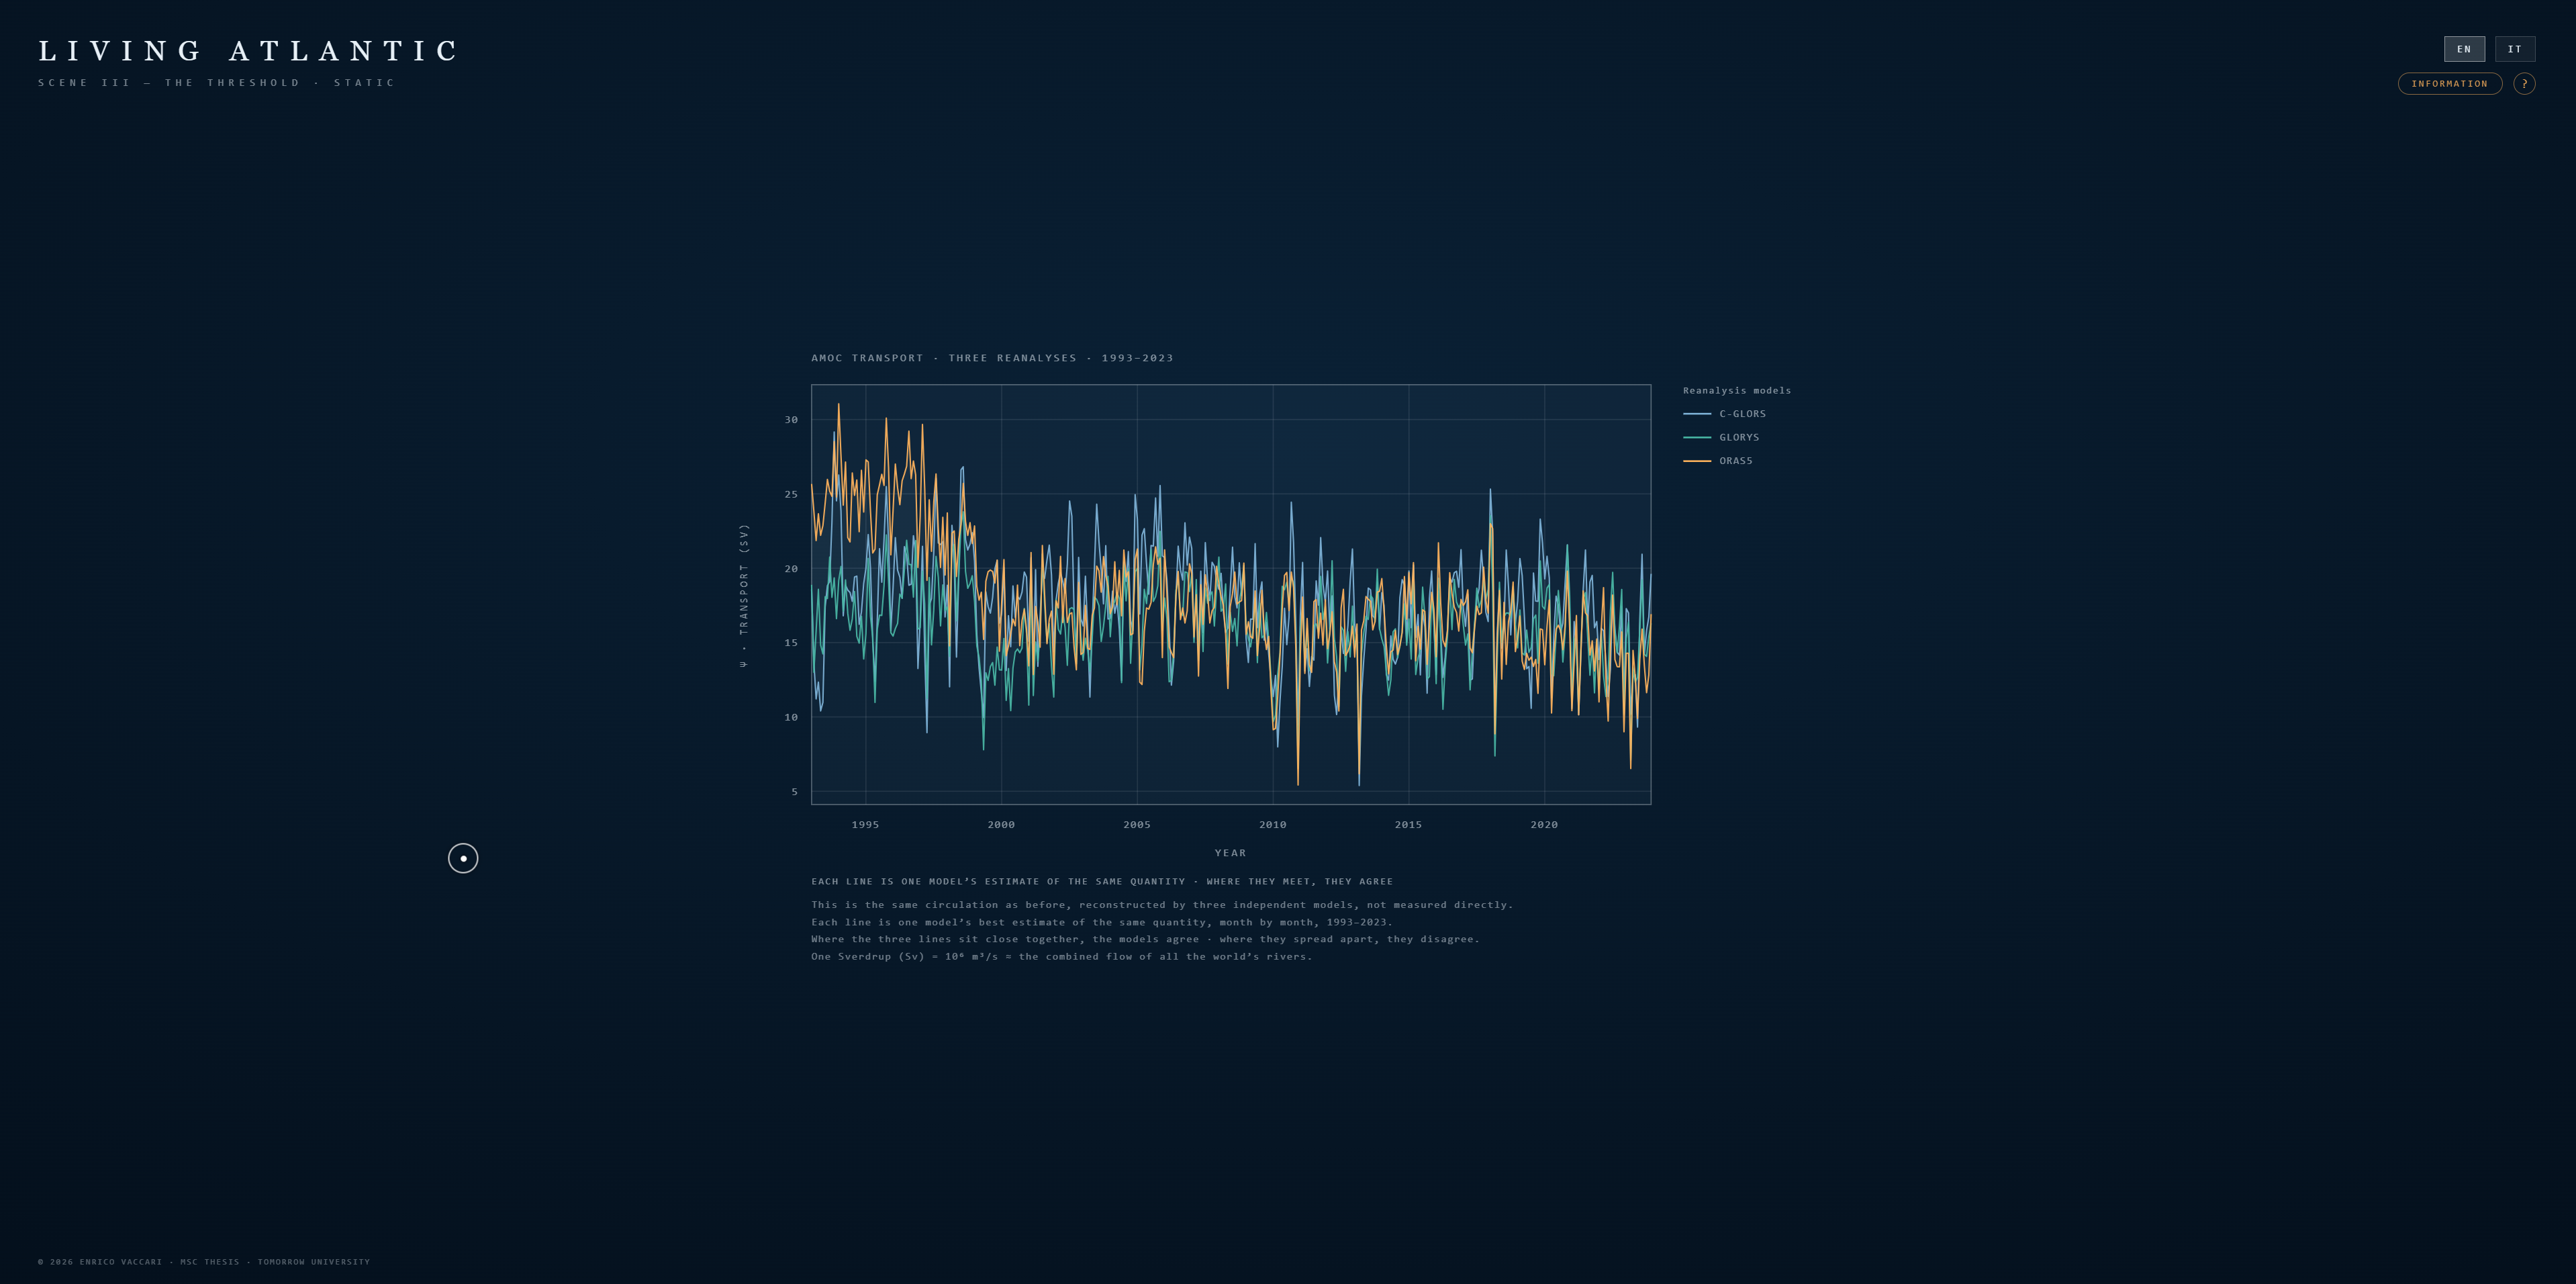
\includegraphics[width=\textwidth]{figures/viz3/viz3_thethreshold-static.png}
    \caption{Controllo (C1): le tre serie di rianalisi, statiche.}
    \label{fig:thethreshold-static}
  \end{subfigure}
  \hfill
  \begin{subfigure}[t]{0.48\textwidth}
    \vspace{0pt}
    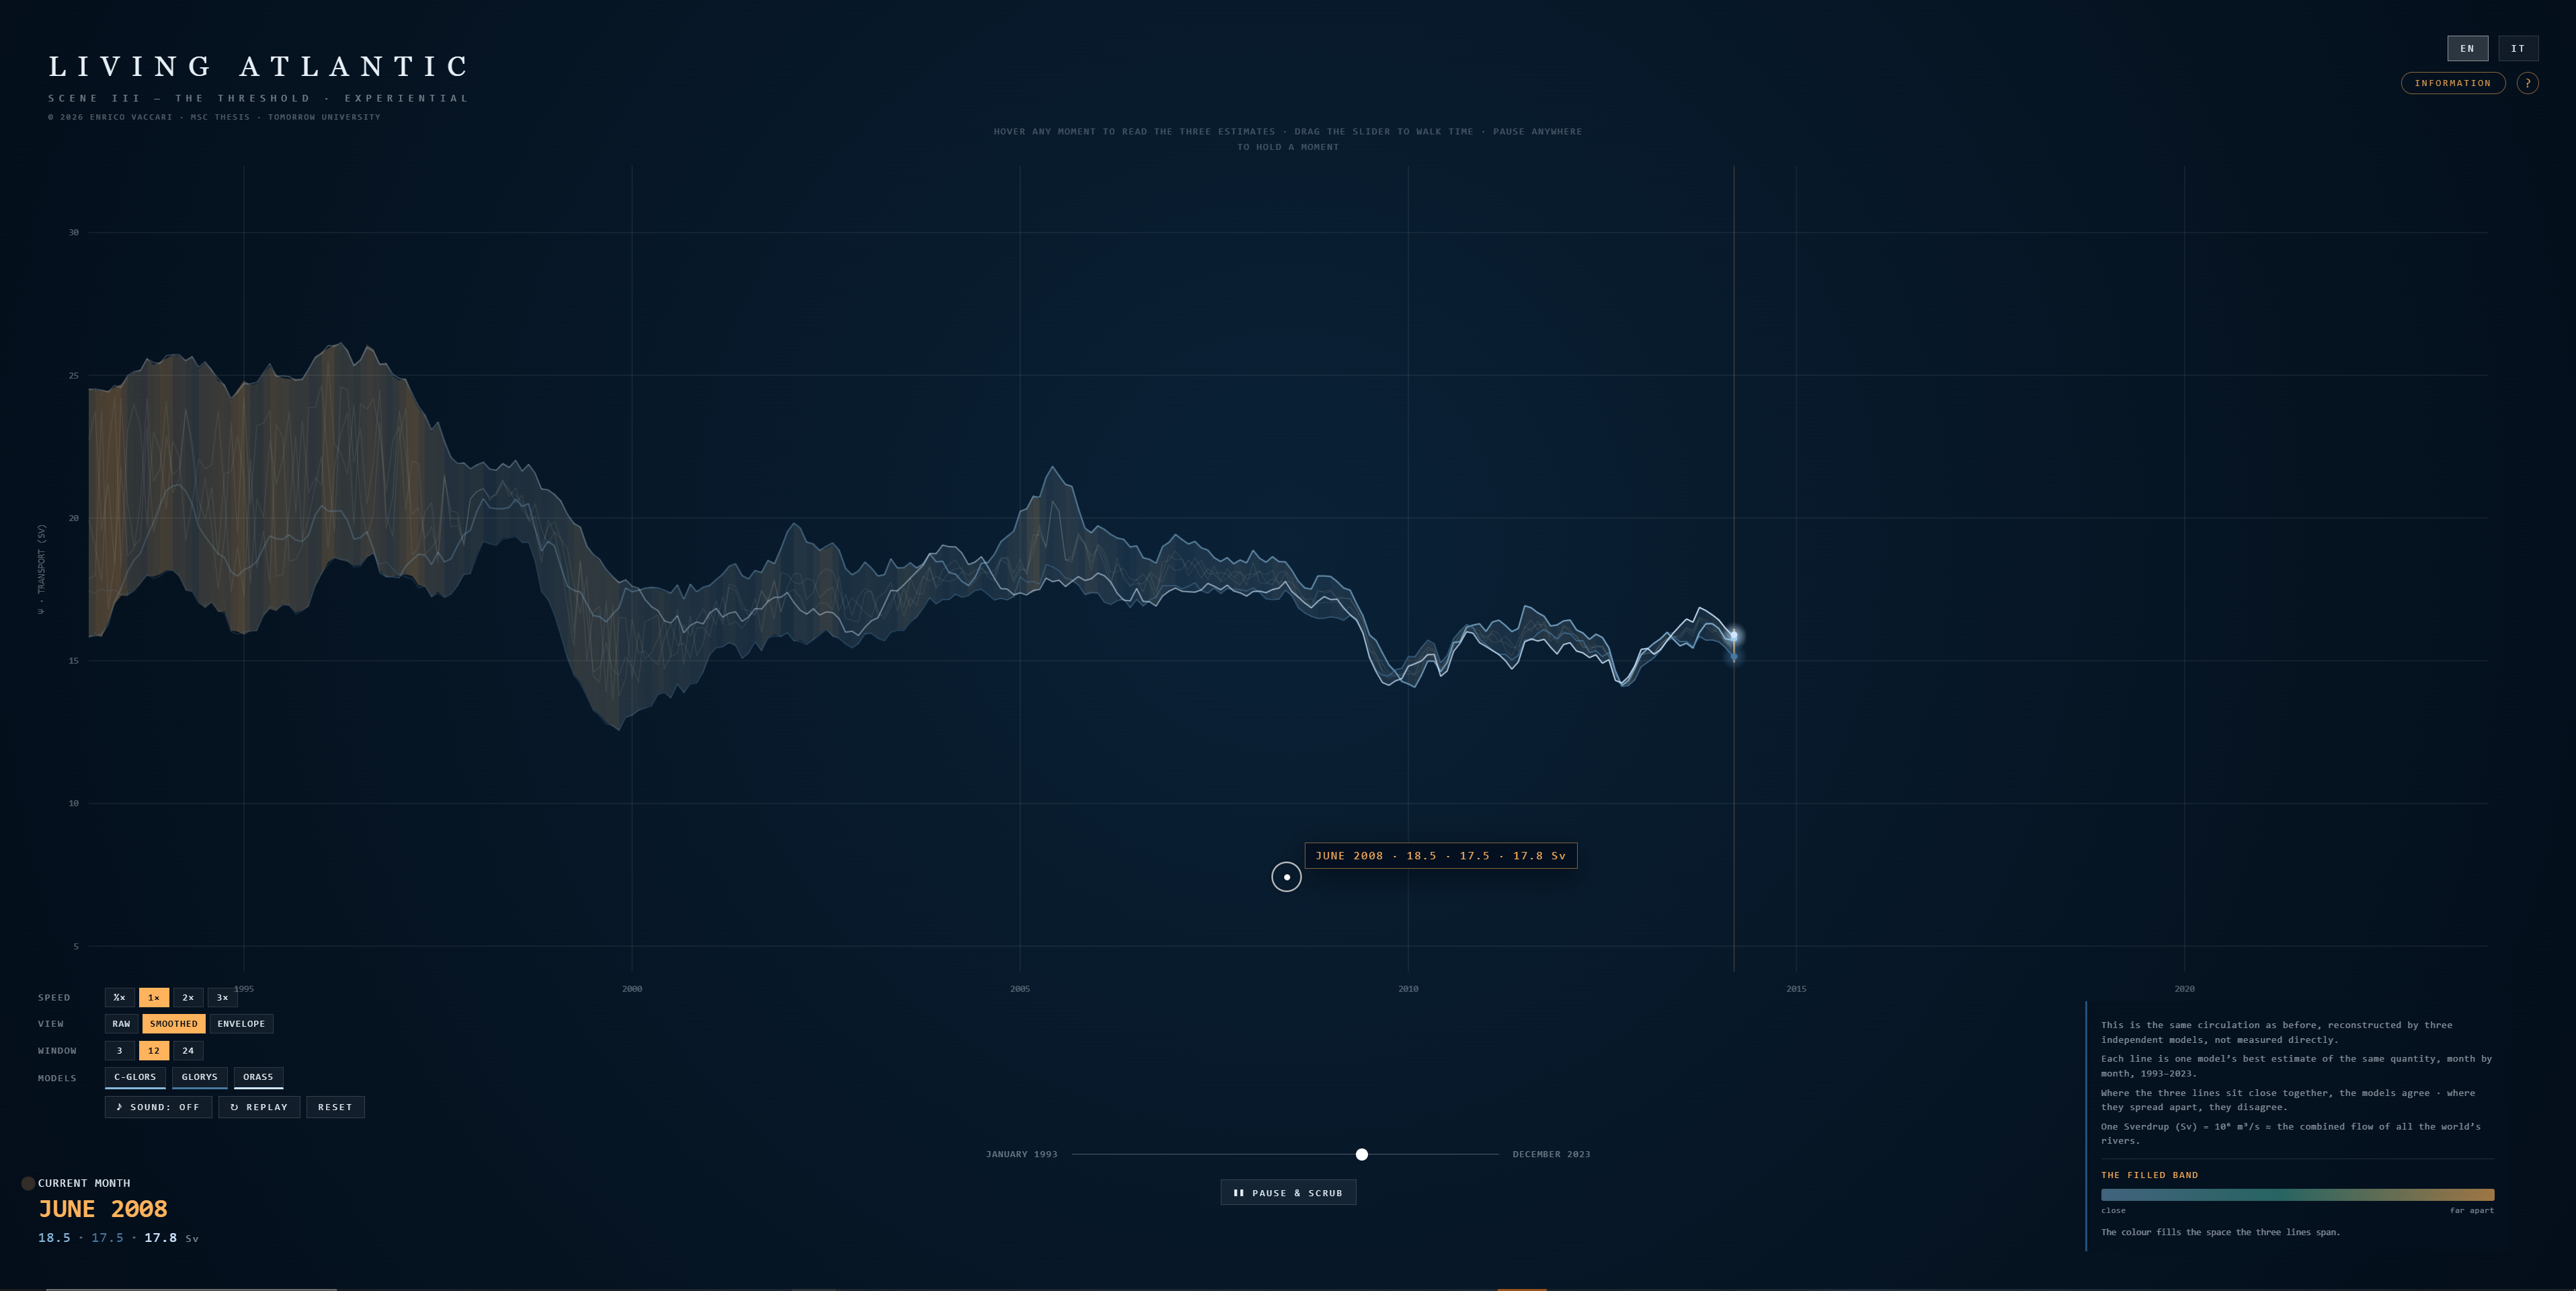
\includegraphics[width=\textwidth]{figures/viz3/viz3_thethreshold-experiential.png}
    \caption{Esperienziale (C2+C3): le stesse serie, con il loro disaccordo reso come movimento.}
    \label{fig:thethreshold-experiential}
  \end{subfigure}

  \caption[Le due condizioni della Scena~III]{Le due condizioni somministrate della
  Scena~III, tratte dagli stessi tre membri di rianalisi Copernicus. La condizione
  statica mostra le tre serie tutte insieme; la condizione esperienziale rende il loro
  disaccordo mutevole come movimento e suono.}

  \label{fig:thethreshold-conditions}
\end{figure}
